\documentclass[10pt]{article}
\usepackage{blindtext}
\usepackage{multicol}
\usepackage[sorting=none, style=nature]{biblatex} 
\usepackage{graphicx}
\usepackage{subcaption}
\usepackage[export]{adjustbox}
\usepackage{wrapfig}
\usepackage{multirow}
\addbibresource{bibliography.bib}
\setlength{\columnsep}{1cm}
\addtolength{\oddsidemargin}{-.875in}
\addtolength{\evensidemargin}{-.875in}
\addtolength{\textwidth}{1.75in}
\addtolength{\topmargin}{-.875in}
\addtolength{\textheight}{1.75in}
\usepackage{hyperref}
\hypersetup{
    colorlinks=true,
    linkcolor=blue,
    filecolor=magenta,      
    urlcolor=cyan,
    citecolor = black,
    pdftitle={Overleaf Example},
    pdfpagemode=FullScreen,
    }

\urlstyle{same}

\title{\textbf{In-Hospital Mortality Prediction for ICU Patients} \\ BIOSTAT 823 Final Project }
\author{Caitlyn Nguyen}
\date{December 16th, 2022 }
\begin{document}
\maketitle
\graphicspath{{images/}}

\begin{multicols}{2}
[
\section{Abstract}
Intensive Care Units (ICUs) are areas within hospitals that provide crucial treatment for critically-ill patients. In this study, we tested three different neural network model architectures to improve prediction for in-hospital mortality of ICU patients. Demographic and routinely collected physiological data from 2001 to 2012 was sourced from the Multiparameter Intelligent Monitoring in Intensive Care III (MIMIC-III) Clinical Database. There were a total of  n = 1,178 individuals. The best model architecture had an AUROC of 0.776 and an AUPRC of 0.600. This model shows the possibility of incorporating both baseline demographic data and medical laboratory for in-hospital mortality prediction. This provides insights on how we can develop clinical decision support tools to aid clinicians in making data-driven decisions when caring for patients.
]

\section{Introduction}
Intensive Care Units (ICUs) are areas within hospitals that provide crucial treatment of critically-ill patients \cite{1}. During an ICU visit, many vital measurements are taken to serve as markers for the patient's health \cite{1}. This data is historically underused and wasted \cite{2}. Machine learning methods can particularly be leveraged to automate the utilization of the rich ICU data and support data-driven clinical decisions. This study seeks to explore different neural network architectures to improve in-hospital mortality prediction for ICU patients. It is important to develop a prediction model that considers all patient information provided from an ICU encounter as a patient-specific clinical decision support tool. With improved predictions, clinicians could use this tool to support their data-driven decisions on
medical treatment and initiate quality of life conversations, impacting the lives of thousands of patients in critical condition.

\section{Data Description}
Demographic and routinely collected physiological data from 2001 to 2012 was sourced from the Multiparameter Intelligent Monitoring in Intensive Care III (MIMIC-III) Clinical Database \cite{3}. The data was collected from the ICU unit of Beth Israel Deaconess Medical Center.  The data was collected, cleaned, and transformed by Sarabh Shahane on Kaggle \cite{4}. In the first 24 hours of each ICU admission the following data were collected: demographic characteristics (age at the time of hospital admission, sex, ethnicity, weight, and height); vital signs (heart rate, (HR), systolic blood pressure [SBP], diastolic blood pressure [DBP], mean blood pressure, respiratory rate, body temperature, saturation pulse oxygen [SPO2], urine output); comorbidities (hypertension, atrial fibrillation, ischemic heart disease, diabetes mellitus, depression, hypoferric anemia, hyperlipidemia, chronic kidney disease (CKD), and chronic obstructive pulmonary disease [COPD]); and laboratory variables (hematocrit, red blood cells, mean corpuscular hemoglobin [MCH], mean corpuscular hemoglobin concentration [MCHC], mean corpuscular volume [MCV], red blood cell distribution width [RDW], platelet count, white blood cells, neutrophils, basophils, lymphocytes, prothrombin time [PT], international normalized ratio [INR], NT-proBNP, creatine kinase, creatinine, blood urea nitrogen [BUN] glucose, potassium, sodium, calcium, chloride, magnesium, the anion gap, bicarbonate, lactate, hydrogen ion concentration [pH], partial pressure of CO2 in arterial blood, and LVEF). Data was transformed to be patient-level, resulting in a total of n = 1,178 individuals. Mean value imputation was done for missing values. The outcome was in-hospital mortality, a binary variable of mortality status at hospital discharge. The prevalence of in-hospital mortality was 0.135. The datafile and all other resources for this project can be found at: \url{https://github.com/caitlynmn/BIOSTAT823_Final_Project}.
 
\section{Data Cleaning}
Prior to modelling, different data cleaning steps were performed in Python. The data had to first be standardized such that all laboratory data were in the scale of [0, 1] as the inputs for the neural network. It was then found that 19 of the 35 laboratory variables had missing values. Mean imputation was done to fill these missing values. One patient had an unknown outcome and was removed from the dataset. The outcome variable was then converted to binary with int64 dtype. The gender variable, originally coded as 1 = Female and 2 = Male, was re-coded to be 0 = Female and 1 = Male. The final dimensions of the data were 1,178 observations across 48 predictors.

\section{Data Splitting}
The data was split into a 80:10:10 ratio of training, validation, and testing datasets. The sample size of the training, validation, and testing datasets were 940, 118, and 118, respectively. The split data was then converted to tensors, with the predictor tensors of the training, validation, and testing datasets being of respective size (940, 48), (118, 48), and (118, 48). The Keras API of TensorFlow was used. Class imbalance was checked and in-hospital mortality was shown to have a prevalence of 0.135, as there were 1017 survivors and 159 non-survivors. To address this, class weights were calculated to give more weight to those observations with an observed in-hospital mortality. The class weights for the survivor class and non-survivor class were 0.575 and 3.821, respectively.

\section{Methods}
Three neural network architectures were constructed using Keras from TensorFlow in Python. The first model had four layers: an input layer, flatten layer, and two dense layers. The input layer had an input of 48 units for the 48 predictors. Inputs are then flattened and passed to a dense layer with 128 hidden units and a Rectified Linear Unit (ReLU) activation function. The final output layer had 1 hidden unit with the sigmoid activation function to return a predicted probability for in-hospital mortality from 0 to 1. The callback of the model was defined to save the model weights at the maximum validation accuracy. The model was compiled using an Adam optimizer with a learning rate of 0.001 using a binary cross-entropy loss function. The monitored evaluation metric of the model was the validation accuracy. The model was trained using 200 epochs with a batch size of 64. Class weights were applied as discussed earlier to adjust for the imbalanced classes. The training and validation accuracy and loss were plotted. The second model used similar architecture to the first model, but instead a dropout layer was added between input layer and the flatten layer. The dropout rate was 0.05. The order of layers in the second model were the input, dropout(0.05), flatten, dense(128), and dense(1) layers. The dense layer was added due to visible overfitting of the first model, which will later be explained in the Results section. The learning rate was also decreased from 0.001 to 0.0001 to slow the learning of the model. Training and validation with the second model was done with 200 epochs and a batch size of 64, the same values for the first model's training. The accuracy and loss on the training and validation sets across epoch were plotted. The third model architecture had two additional dense layers and increased dropout layer. The architecture then became: input, dropout(0.1), flatten, dense(128), dense(64), dense(32), and dense(1). The two additional dense layers with 64 and 32 hidden units, respectively, were added to increase the complexity of the model to address slight potential for underfitting. To slightly offset the added complexity of the model, the dropout rate was increased from 0.05 to 0.1. The learning rate remained at 0.0001. The model was then trained across 200 epochs with a batch size of 64 again. Plots of the loss and accuracy were again produced. The final model to be used on the testing dataset was evaluated by both the accuracy and loss metrics of the validation dataset, and examination of the evaluation plots. The best model's weights at the maximum validation accuracy were loaded. The testing dataset was used to produce the predicted probability for in-hospital mortality. The accuracy, Receiver-Operator Curve, area under the Receiver-Operator Curve (AUROC), Precision-Recall curve, area under the Precision-Recall Curve, and confusion matrix with corresponding evaluation metrics of sensitivity, specificity, precision, negative predictive value, and F1-score were evaluated from the outputs of the final model.

\section{Results}
The training and validation accuracy of model 1 are shown in Figure 1. The resultant loss is shown in Figure 2. The best validation accuracy was observed to be 0.873 at epoch 164. The Accuracy vs Epoch plot 13 shows that there is overfitting observed beginning at epoch 70 because following that epoch, the validation accuracy plateaus while the training accuracy continues to increase. Overfitting is observed with the Loss vs Epoch plot. At around epoch 20, the validation loss begins to plateau while the training loss continues to decrease.

\begin{center}
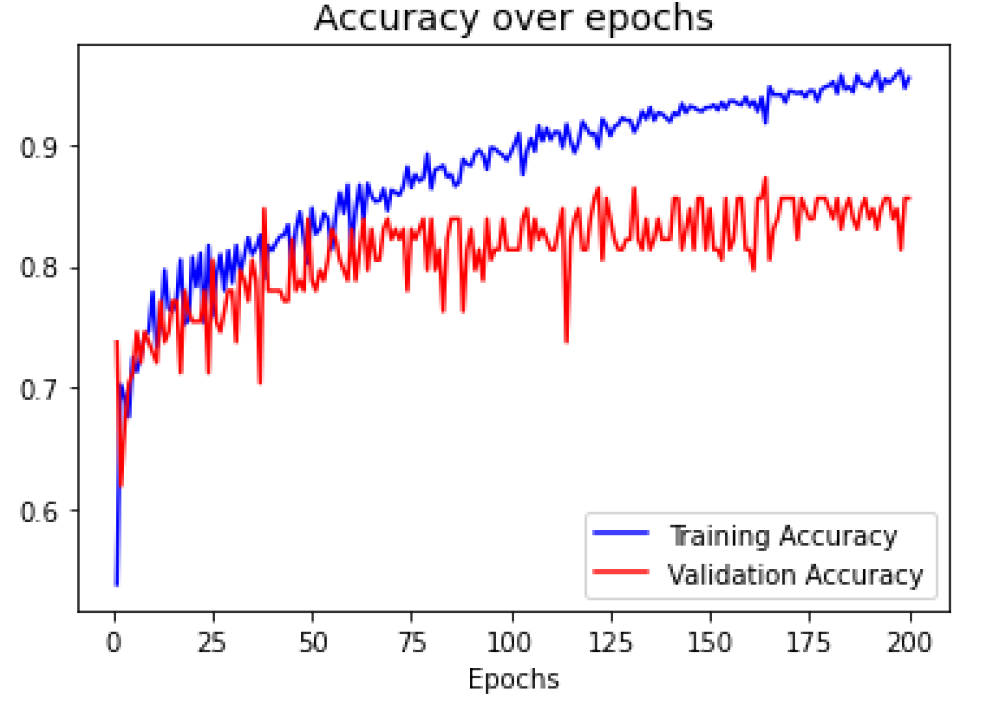
\includegraphics[width=.4\textwidth]{Model1Acc}
    \captionof{figure}{Model 1 Training/Validation Accuracy}
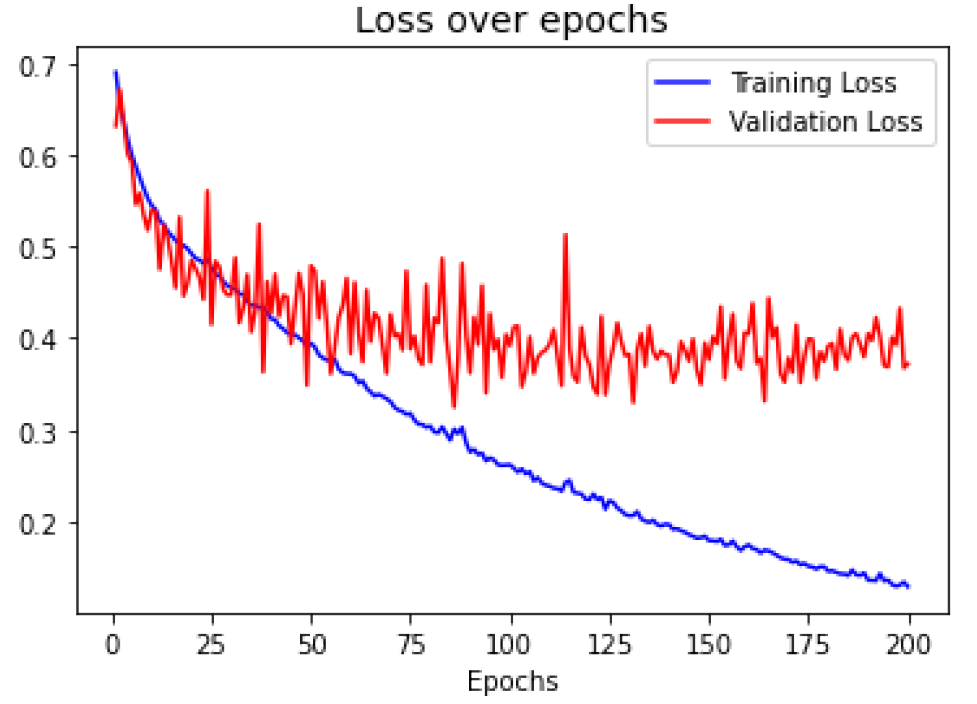
\includegraphics[width=.4\textwidth]{Model1Loss}
    \captionof{figure}{Model 1 Training/Validation Loss}
\end{center}

The accuracy and loss results of model 2 are shown in Figures 3 and 4, respectively. The best accuracy for the validation set was 0.780 at epoch 114. This validation accuracy is worse than the first validation accuracy of 0.873 which occurred at epoch 164. It appears that the training and validation accuracy have plateau'd around 0.750. Both losses are still decreasing (although validation is decreasing at a slower rate), indicating that there is underfitting and more training can be done to reach the optimum solution.

\begin{center}
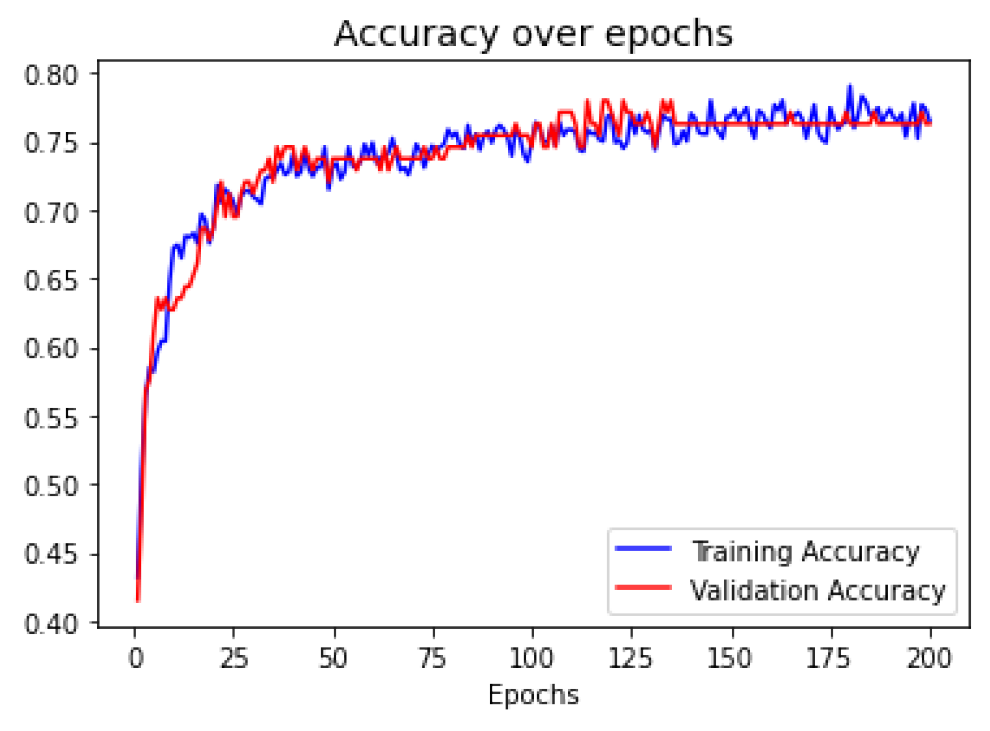
\includegraphics[width=.4\textwidth]{Model2Acc}
    \captionof{figure}{Model 2 Training/Validation Accuracy}
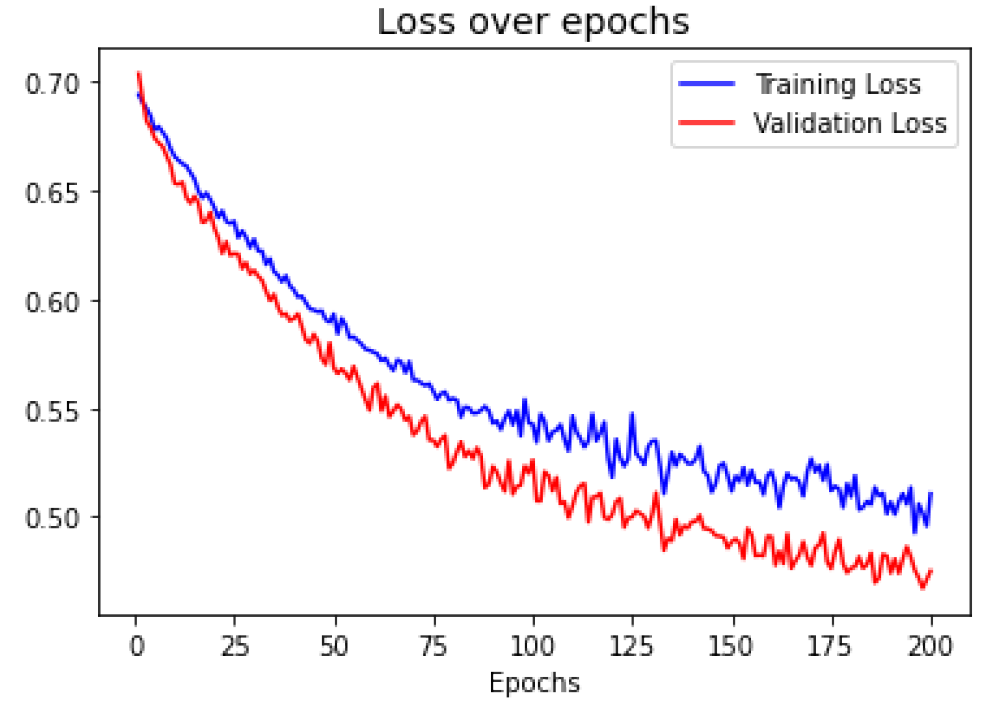
\includegraphics[width=.4\textwidth]{Model2Loss}
    \captionof{figure}{Model 2 Training/Validation Loss}
\end{center}

The accuracy and loss results of model 3 are shown in Figures 5 and 6, respectively. The best validation accuracy was 0.831 at epoch 186. This was less than the validation accuracy of the first model architecture (0.873 at epoch 164), but greater than the validation accuracy of the second model architecture (0.780 at epoch 114). The accuracies began high, most likely due to chance in the mini-batches, and then decreased. Shortly afterwards, the accuracies began to increase. The validation accuracy and training accuracy appear to be similar. More training time could potentially be done as the accuracies appear to potentially continue increasing. The validation loss was consistently below the training loss. There could be potential for more training if there were more epochs.

\begin{center}
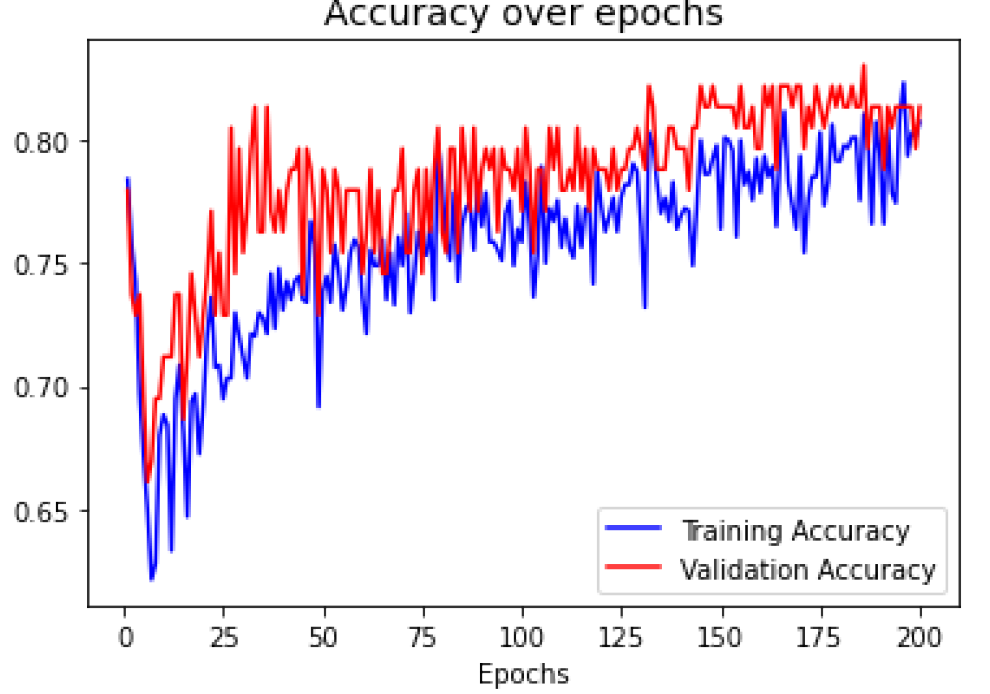
\includegraphics[width=.4\textwidth]{Model3Acc}
    \captionof{figure}{Model 3 Training/Validation Accuracy}
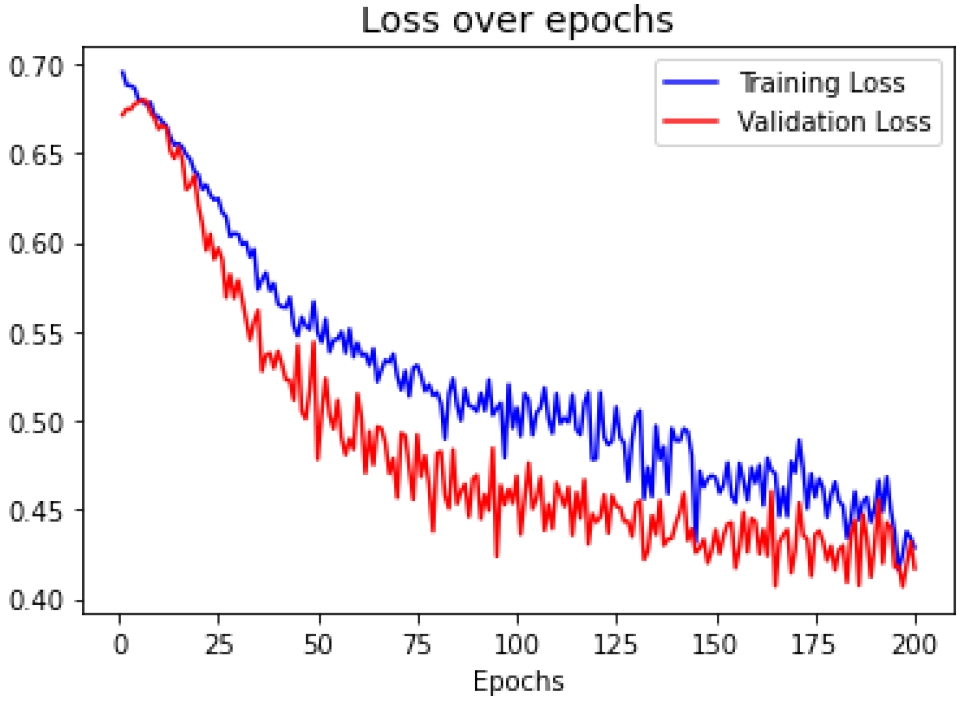
\includegraphics[width=.4\textwidth]{Model3Loss}
    \captionof{figure}{Model 3 Training/Validation Loss}
\end{center}
The resulting training and validation accuracy and loss are reported in Table 1. Model 1 had a maximum validation accuracy of 0.873 with a validation loss of 0.332. Model 2 had a maximum validation accuracy of 0.780 with a validation loss of 0.498. Model 3 had a maximum validation accuracy of 0.831 with a validation loss of 0.444. Model 1 had the highest accuracy and lowest loss for both the training and validation dataset among the models. Model 3 performed the second best, whereas Model 2 had the lowest scores. However, when assessing the plots earlier, Model 1 had the most overfitting, as discussed earlier. Model 3 was chosen as the best model as it had the second best performance, and did not appear to be overfit as much as Model 1.

\begin{center}
\begin{tabular}{ |c||c|c|c|  }
 \hline
 Metric & Model 1 & Model 2 & Model 3\\
 \hline
 Training Acc. & 0.9181 & 0.759 & 0.811\\
 Validation Acc. & 0.873 & 0.780 & 0.831\\
 Training Loss & 0.169 & 0.535 & 0.444\\
 Validation Loss & 0.332 & 0.498 & 0.407\\
 \hline
\end{tabular}
\captionof{table}{Accuracy and Loss of Models}
\end{center}

The weights from when model 3 had achieved its maximum validation accuracy were used with model 3's architecture to evaluate performance on the test dataset. The resulting accuracy on the the test dataset was 0.814. The Receiver-Operator Curve (ROC) is shown in Figure 7. Its resultant area under the curve (AUROC) was 0.776. The Precision-Recall Curve (PRC) is shown in Figure 8 and reported with an area under the curve (AUPRC) of 0.600. The confusion matrix with a classification threshold of 0.5 for the probability is shown in Table 2. This corresponds to a sensitivity of 0.588, specificity of 0.852, precision of 0.400, negative predictive value of 0.925, and a F1-score of 0.476.

\begin{center}
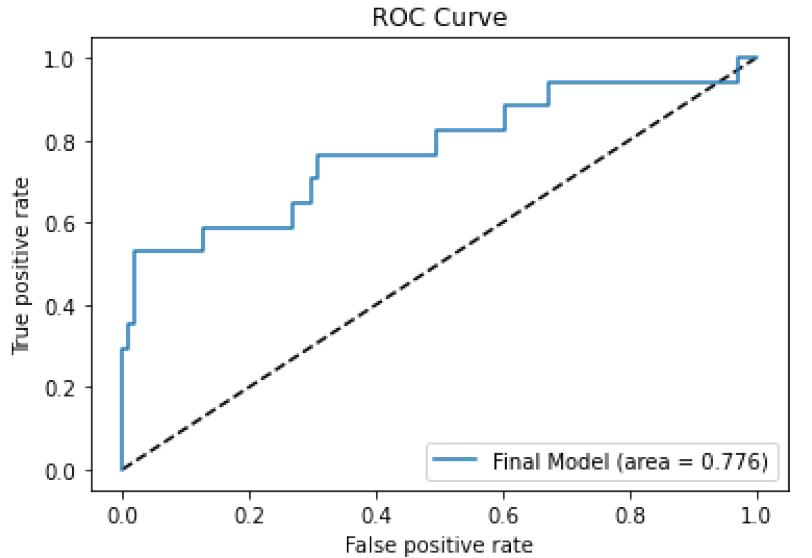
\includegraphics[width=.4\textwidth]{ROC}
    \captionof{figure}{Receiver-Operator Curve (ROC)}
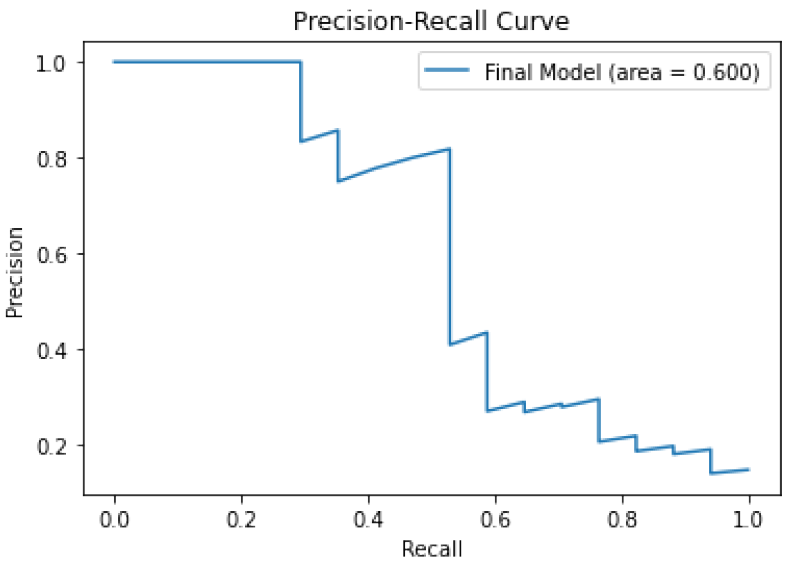
\includegraphics[width=.4\textwidth]{PRC}
    \captionof{figure}{Precision-Recall Curve (PRC)}
\end{center}

\begin{center}
\begin{tabular}{ |c||c|c|  }
 \hline
 & Actually + & Actually -\\
 \hline
 Predicted + & 10 & 15\\
 Predicted - & 7 & 86\\
 \hline
\end{tabular}
\captionof{table}{Confusion Matrix}
\end{center}

\section{Discussion}
The third model was shown to be the best due to high performance and less overfit than the first model. Adding a dropout layer from model 1 to model 2 decreased overfitting, as it prevented the model from co-adapting among neurons. Adding dense layers from model 2 to model 3 helped add more complexity to the model to achieve higher accuracy and decreased loss. Less overfitting is desired as the model would be more generalizable to other datasets and hospitals. This would enable application of the model to reach more hospitals and essentially aid more clinicians in making clinical decisions. The resultant AUROC of 0.776 indicates that the model had a high ability to discriminate between the survivor and non-survivor classes in its predicted probability for in-hospital mortality. The ROC curve showed improvement from the baseline AUROC of 0.5. The PRC also showed improve from the baseline, as the AUPRC was 0.600. This is greater than a 3-fold increase from the prevalence of in-hospital mortality in the testing set, which was 0.212. This shows that the model was able to handle the positive cases (non-survivors) relatively well, given the class imbalance. For baseline analysis, a classification threshold of 0.5 was used, where a predicted probability greater than 0.5 would be classified as non-survivor and a predicted probably less than or equal to 0.5 would be classified as survivor. The sensitivity was slightly greater than random, showing that the model did not increase detection rate by much when the class was actually non-survivor. The model did well in classifying the true negatives, shown with its high specificity. It should be discussed with clinicians which threshold would be best for the application of this model, as the overall performance from the ROC and PRC deemed well, but using a classification threshold of 0.5 does not maximize the predictive performance of the model. It should be noted that the sample size of the testing set was only n = 118 with 25 non-survivors and 93 survivors. The prevalence of in-hospital mortality was 0.212 in this testing set, whereas in the whole dataset, it was 0.135. This difference in proportion of cases in the testing dataset as opposed to what the model was trained on could have led to the high false negative rate of 0.412 and the low sensitivity of 0.588. Additionally, hyperparameter tuning of the learning rate, batch size, and number of epochs was not done beyond using inspection to determine if it needed to be changed across the three models.

\section{Conclusion}
The neural network architecture with more dense layers and a dropout layer with a greater dropout rate showed to have the best performance, as it had a balance of accuracy and generalization. The model showed great discrimination between the survivors and non-survivors, and potential for correctly classifying non-survivors. The classification threshold at which to classify non-survivor vs survivor from the predicted probability should be discussed with clinicians. This would help provide further evaluation metrics on the predictive capability of the model, rather than using a default threshold of 0.5. Hyperparameterization can also be done via grid search to determine the optimum learning rate, batch size, and number of epochs for the model. Other machine learning models could be evaluated with this data, such as a regularized logistic regression, random forest, and support vector machine, to determine differences in performance across models. These efforts to improve in-hospital mortality for ICU patients could bridge the gap between clinicians and medical data, enabling the clinicians to make patient-specific clinical decisions to improve the life of their patients.

\end{multicols}
\printbibliography
\end{document}